\documentclass[12pt, a4paper]{report}
%\usepackage[utf8]{inputenc} 
\usepackage{fullpage}
\usepackage{amssymb}
\usepackage{graphicx}
\usepackage[hidelinks]{hyperref}
\usepackage{xcolor}
\renewcommand\UrlFont{\color{blue}\rmfamily}

\usepackage[backend=biber]{biblatex}
\usepackage{csquotes} % smart quotes + tight integration with biblatex
% Custom bibliography file
\addbibresource{library.bib} 

\usepackage{float}

\usepackage{pgfplots}
\pgfplotsset{compat=1.18}
\usetikzlibrary{arrows.meta}

% Must compile the document with -shell-escape
% Must compile the document in an environment where the `pygments` library is installed in Python
%\usepackage{minted}

% Source code highlighting BEGIN
\usepackage{listings}
\lstset{basicstyle=\small,defaultdialect=[11]c++,frame=lines,numbers=left,numberstyle=\tiny,tabsize=2}
% YAML highlighting hack BEGIN
% Courtesy of Stackoverflow: https://tex.stackexchange.com/a/152856/179871

\newcommand\YAMLcolonstyle{\color{red}\mdseries}
\newcommand\YAMLkeystyle{\color{black}\bfseries\smallfont}
\newcommand\YAMLvaluestyle{\color{blue}\mdseries}
% YAML highlighting hack END


% Landscape-oriented tables
\usepackage{rotating}
\usepackage{booktabs}

\makeatletter

% here is a macro expanding to the name of the language
% (handy if you decide to change it further down the road)
\newcommand\language@yaml{yaml}

\expandafter\expandafter\expandafter\lstdefinelanguage
\expandafter{\language@yaml}
{
	keywords={true,false,null,y,n},
	keywordstyle=\color{darkgray}\bfseries,
	basicstyle=\YAMLkeystyle,                                 % assuming a key comes first
	sensitive=false,
	comment=[l]{\#},
	morecomment=[s]{/*}{*/},
	commentstyle=\color{purple}\ttfamily,
	stringstyle=\YAMLvaluestyle\ttfamily,
	moredelim=[l][\color{orange}]{\&},
	moredelim=[l][\color{magenta}]{*},
	moredelim=**[il][\YAMLcolonstyle{:}\YAMLvaluestyle]{:},   % switch to value style at :
	morestring=[b]',
	morestring=[b]",
	literate =    {---}{{\ProcessThreeDashes}}3
	{>}{{\textcolor{red}\textgreater}}1     
	{|}{{\textcolor{red}\textbar}}1 
	{\ -\ }{{\mdseries\ -\ }}3,
}

% switch to key style at EOL
\lst@AddToHook{EveryLine}{\ifx\lst@language\language@yaml\YAMLkeystyle\fi}
\makeatother

\newcommand\ProcessThreeDashes{\llap{\color{cyan}\mdseries-{-}-}}
% YAML highlighting hack END
% Source code highlighting END


% Title of your project
\title{Fuzzy-Genetic Hybrid Models for Large-Horizon Deterministic Planning}

% Name of deliverable
\newcommand{\deliverableName}{Final Master’s Project}

% Group names(s)
\author{Mark Safronov}

% Advisor
\newcommand{\directedBy}{Dr. Jordi Duch}

% Group number
\newcommand{\groupNumber}{A\_2024-25\_105200}

% Any comments for us
\newcommand{\comments}{Comments for teachers of the course}

% Web address for the project (if any)
\newcommand{\homepage}{\url{https://campusvirtual.urv.cat/course/view.php?id=105200}}

% Date for title page, default is today and 
\date{\today}


\makeatletter{}

\begin{document}
	
	% Title page based on https://www.latextemplates.com/template/academic-title-page
\begin{titlepage}
	\newcommand{\HRule}{\rule{\linewidth}{0.3mm}} % Defines a new command for horizontal lines, change thickness here
	\center % Centre everything on the page
	%------------------------------------------------
	%	Headings
	%------------------------------------------------
	
	\textsc{\LARGE Universitat Rovira i Virgili}\\[1.5cm]
	
	\textsc{\Large \deliverableName}\\[0.5cm]
	
	\textsc{\large Masters of Artificial Intelligence and Computer Security}\\[0.5cm]
	
	%------------------------------------------------
	%	Title
	%------------------------------------------------
	
	\HRule\\[0.4cm]
	
	{\huge\bfseries \@title}\\[0.4cm]
	
	\HRule\\[1.5cm]
	
	%------------------------------------------------
	%	Author(s)
	%------------------------------------------------
	
	% 	If you don't want a supervisor, uncomment the two lines below and comment the code above
	%	{\large\textit{Author}}\\
	{\large\sc\@author} % Your name
	
	%------------------------------------------------
	%	Date
	%------------------------------------------------
	
	\vfill\vfill
	{\large\@date} % Date, change the \today to a set date if you want to be precise
	\vfill\vfill\vfill
	
	%   \footnotesize{Comments: \comments}
	%   \vfill\vfill
	%    \homepage
	%    \vfill
	
	%------------------------------------------------
	% Change log for the plan (can be deleted before delivery)
	% When you update the plan please record what you changed and what the reason for the change. This will be useful for your supervisor.
	%------------------------------------------------
	% \input{./changelog.tex}
	
	%------------------------------------------------
	%	Logo
	%------------------------------------------------
	\vfill
	
\includegraphics[width=0.3\textwidth]{./urvlogo.png}
	\vfill
	
	
\end{titlepage}

	
	\begin{abstract}
		This thesis investigates the problem of deterministic planning with long horizons, where an agent must execute a fixed-length sequence of actions that transform its state into a desired goal state. Such problems arise in domains ranging from robotics to scheduling, and are characterized by a combinatorial explosion of possible trajectories.
		
		The motivating case study is the Japanese life simulation game Princess Maker 2, which, when stripped of its narrative elements, yields a formal instance of this problem: an agent described by dozens of numeric attributes, several dozen actions, and a planning horizon of thousands of steps. Classical approaches such as automatic planning and reinforcement learning fail to scale under these conditions, either due to incompatibility with fixed-horizon evaluation or due to the curse of dimensionality and sparse terminal rewards.
		
		To address this, we propose a hybrid heuristic method that combines fuzzy logic and genetic algorithms. Domain knowledge is encoded as fuzzy rules, which reduce the effective dimensionality of the problem by introducing latent parameters called inclinations. These inclinations are optimized by evolutionary algorithms, turning the original intractable search into a manageable optimization task.
		
		We implement this method using the fuzzylite and pagmo libraries in C++, and evaluate it on test cases of increasing complexity. Results show that the solver is able to construct valid action sequences that satisfy predefined goal conditions, with runtime scaling linearly with the planning horizon. While the manual design of fuzzy rules remains a limitation, the proof of concept demonstrates that fuzzy-genetic heuristics can effectively solve large-horizon deterministic planning problems, where classical methods are impractical.
	\end{abstract}
	\tableofcontents
	
	\chapter{Introduction}
	
	\section{Motivation and Context}
	
	A deterministic planning problem for a stateful agent is one of the most generic formulations in artificial intelligence. 
	The task can be summarized as selecting a sequence of actions which transforms the state of an agent into a desired goal state. 
	This formulation naturally appears in a wide range of real-world domains: robotics (planning robot trajectories under resource and time constraints), industrial scheduling (allocating tasks to maximize production while minimizing downtime), and control systems (maintaining stability of dynamic processes under changing conditions).
	
	The key difficulty in such problems is the combinatorial explosion. 
	As soon as the number of available actions grows and the planning horizon becomes long, the search space of all possible trajectories expands exponentially. 
	This phenomenon, commonly referred to as the curse of dimensionality, renders classical exhaustive approaches infeasible even for moderately sized problems.
	
	Works like~\cite{WOS:001308319900003} cover both the real-world applications and a significance of the curse of dimensionality.
	
	In this work, we use the Japanese computer game Princess Maker 2 (Gainax, 1993) as a motivating case study. 
	While the game itself is narrative-driven and contains many mechanics that go beyond formal modeling, its core gameplay loop is a textbook instance of a deterministic planning problem. 
	The player controls a stateful agent — the daughter character — by repeatedly selecting actions such as study, work, or leisure. 
	Each action deterministically modifies a set of numerical attributes, and after a fixed horizon of in-game years, the outcome is evaluated against predefined conditions that determine the “ending.”
	
	In the appendix~\ref{appendix::screenshots} two screen captures are presented to demonstrate the complexity of the character attributes encoding and the action space in this game.
	
	Stripped of its narrative elements, Princess Maker 2 yields a highly formal planning problem: an agent with dozens of numeric attributes, several dozen possible actions, and a planning horizon of several thousand steps. 
	This combination of a large state space, broad action set, and long horizon exemplifies the type of problem where classical planners and reinforcement learning approaches both struggle. 
	At the same time, because the formulation is generic, any progress on this problem carries implications well beyond the original game context.
	
	In the following section we will briefly review the most obvious approaches to this problem, namely, automatic planning theory and reinforcement learning, and discuss why they both fail to scale to the case we are interested in.
	
	\section{Existing Approaches}\label{section::existing-approaches}
	
	\subsection{Automatic Planning Theory}
	
	Automatic planning in artificial intelligence is historically grounded in the STRIPS~\cite{fikes1971strips} formalism, which defines planning as the composition of operators that transform an initial world model into one satisfying a goal condition.
	In principle, this description matches exactly the type of solver we are aiming for: we have a stateful agent, a set of deterministic actions, and a requirement to reach a specified goal state.
	
	Modern planners, such as ENHSP~\cite{enhsp::scala2020subgoaling}~\cite{enhsp::Scala2016IntervalBasedRF}, extend this formalism to support numeric fluents and continuous effects. 
	On small-scale problems they have been demonstrated to work effectively, often guaranteeing optimality of the resulting plan.
	For example, existing benchmarks~\footnote{\url{https://github.com/hstairs/enhsp/tree/enhsp-20}} include instances with up to forty numeric variables and around ten actions, which can be solved in practical time.
	
	However, the core assumptions of classical planning diverge from the requirements of our case.
	Most planners are designed to minimize plan length, i.e., to find the shortest action sequence that satisfies the goal.
	In contrast, the Princess Maker 2 formulation requires executing a fixed number of steps before the final state can be evaluated.
	No-operation actions are not available, so every step transforms the agent’s state irreversibly.
	This means that reaching the goal “too early” is not valid — it is only the state after the full horizon that determines success.
	
	In addition, the problem of scale remains prohibitive.
	Even if the goal condition could be reformulated to suit the planner’s semantics, the state space induced by 23 attributes, 27 actions, and thousands of steps is far outside the scope of tractable automatic planning.
	Research does exist on scaling planners with temporal logics~\cite{LU2025121666} and heuristics, but these approaches are not focused on high-dimensional numeric fluents of the type present in our motivating case.
	
	\subsection{Reinforcement learning}
	
	Reinforcement learning~\cite{sutton2018reinforcement} (RL) is another approach which seems, at first glance, to be a natural fit for the problem.
	In RL, we model an agent interacting with an environment: the agent observes a state, selects an action, and receives a reward.
	Over time, the agent is expected to learn a policy that maximizes cumulative reward.
	The analogy with our setting is straightforward — the state is the character’s attributes, the actions are the available schedule choices, and the “reward” is the final outcome at the end of the planning horizon.
	
	However, the practical obstacles are significant.
	The first is the dimensionality of the state space.
	With 23 attributes each taking values in the range of roughly 0 to 500, the number of possible states is astronomically large.
	A naive tabular representation of a Q-function would require a table of size $27 \times 500^{23}$, which is intractable to store or update.
	While function approximation can reduce this requirement, it does not remove the exponential blowup inherent in such spaces.
	
	The second issue is the length of the planning horizon.
	In the simplified gameplay setup, the player makes three choices per month for ten in-game years, which already leads to a search tree over 360 steps.
	In the full day-by-day formulation the horizon is an order of magnitude longer.
	Standard RL algorithms struggle when the reward is sparse and delayed, as in this case where only the terminal state matters.
	Exploration becomes ineffective because the probability of randomly reaching a good ending within thousands of steps is vanishingly small.
		
	Finally, unlike in many RL benchmarks, our problem does not allow neutral or reversible actions.
	Every action irreversibly changes the state, which exacerbates the exploration problem.
	Taken together, these aspects make classical reinforcement learning algorithms impractical for the problem scale we consider.

	\section{Fuzzy Logic and Fuzzy Controllers}
	
	Fuzzy logic, introduced by L. Zadeh in 1965, extends classical set theory by allowing partial membership of elements in a set.
	Instead of a variable belonging to a set either completely or not at all, in fuzzy logic a variable may belong to a set with a degree between 0 and 1.
	This allows us to model linguistic terms such as “low,” “medium,” or “high” in a mathematically precise way.
	
	A fuzzy controller applies this idea to decision-making.
	The system is defined through linguistic variables with associated membership functions, and a collection of symbolic rules.
	A typical example outside this work would be:
	
\begin{verbatim}
	If temperature is high then fan speed is high.
\end{verbatim}
	
	Here, both “temperature” and “fan speed” are fuzzy variables, and the rule connects them in a way that corresponds directly to human reasoning.
	After applying fuzzification (mapping numeric input values into fuzzy terms), rule evaluation, and defuzzification (converting fuzzy outputs back into numeric values), the controller produces an actionable decision.
	
	The benefit of this approach is the ability to capture domain knowledge without enumerating every possible combination of numeric parameters.
	Instead of constructing a complete reward table or transition map — which would be infeasible in large state spaces — we specify a relatively small set of symbolic rules which generalize across many states.
	This makes fuzzy controllers attractive for problems where expert intuition about the domain exists, but exhaustive specification is impossible.
	
	In the context of this work, fuzzy controllers provide a mechanism to express priorities over actions in symbolic terms, forming a bridge between human-understandable heuristics and algorithmic decision-making.
	
	\section{Genetic Algorithms}
		
		Genetic algorithms~\cite{song2023rl_ea}~\cite{beyer2002evolution_strategies} (GAs) are a class of optimization methods inspired by biological evolution.
		A population of candidate solutions is maintained, where each solution is represented as a genome — a sequence of values encoding the parameters of interest.
		The algorithm proceeds iteratively through the following steps:
		
		\begin{enumerate}
			\item Evaluation: every genome is assigned a fitness score according to an objective function.
		
		\item Selection: genomes with higher fitness are more likely to be chosen for reproduction.
		
		\item Crossover: pairs of genomes exchange parts of their structure, creating new offspring that combine traits of both parents.
		
		\item Mutation: with low probability, individual genes are randomly altered, introducing diversity.
		
		\item Replacement: the new generation replaces the old, and the process repeats.
		\end{enumerate}
		
		Over time, the population tends to evolve towards fitter solutions, even when the search space is large, non-linear, or poorly understood. The method does not guarantee a globally optimal solution, but it often finds good approximations in domains where exact methods are computationally infeasible.
		
		The main advantage of GAs is that they treat the problem as a black box: only the ability to evaluate candidate solutions is required, while no assumptions about continuity, differentiability, or convexity are needed. This makes them well suited for combinatorial or highly non-convex problems.
		
		In the context of this work, genetic algorithms will be used to optimize the inclinations — latent behavioral parameters that guide the fuzzy controller. This reduces the original planning problem from direct search over long sequences of actions to an evolutionary search in a much smaller parameter space.
	
	\section{Our Proposed Approach}
	
	The discussion in the section~\ref{section::existing-approaches} shows that classical approaches such as automatic planning or reinforcement learning are unable to scale to the requirements of our motivating problem. To address this, we propose a hybrid heuristic method which combines symbolic reasoning with evolutionary optimization.
	
	The core idea is to replace direct search over complete action sequences with search over a smaller set of latent behavioral parameters, which we call inclinations. These inclinations represent tendencies toward particular groups of actions. A fuzzy controller then maps the inclinations together with the current state into a concrete choice of action.
	
	This formulation has two benefits. First, it allows us to encode domain knowledge directly into the fuzzy rule base, reducing the effective dimensionality of the search. Second, it enables optimization to take place in the smaller inclination space, rather than in the exponentially large space of all possible trajectories. The resulting search problem becomes tractable for evolutionary algorithms such as genetic algorithms, which only require evaluation of candidate solutions, not explicit enumeration of the search space.
	
	The hypothesis of this work is that such a hybrid fuzzy-genetic approach can find valid solutions in polynomial-like time in cases where reinforcement learning or automatic planners fail due to combinatorial explosion.
	
	The overall process is illustrated in Figure~\ref{fig:approach-diagram}.
	
	\begin{figure}[H]
		\centering
		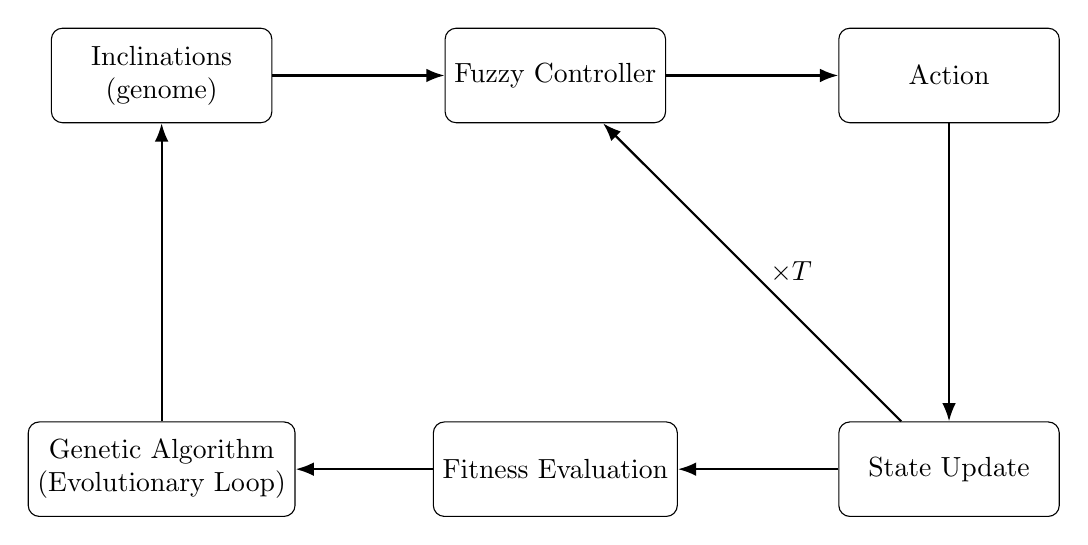
\begin{tikzpicture}[node distance=5cm, auto, >=Latex]
			
			% Styles
			\tikzstyle{block} = [rectangle, draw, rounded corners, minimum height=1.2cm, minimum width=2.8cm, align=center]
			\tikzstyle{arrow} = [->, thick]
			
			% Nodes
			\node[block] (inclinations) {Inclinations \\ (genome)};
			\node[block, right of=inclinations] (fuzzy) {Fuzzy Controller};
			\node[block, right of=fuzzy] (action) {Action};
			\node[block, below of=action] (state) {State Update};
			\node[block, left of=state] (fitness) {Fitness Evaluation};
			\node[block, below of=inclinations] (evolution) {Genetic Algorithm \\ (Evolutionary Loop)};
			
			% Arrows (main flow)
			\draw[arrow] (inclinations) -- (fuzzy);
			\draw[arrow] (fuzzy) -- (action);
			\draw[arrow] (action) -- (state);
			\draw[arrow] (state) -- (fitness);
			\draw[arrow] (state) -- (fuzzy) node[above,midway,right=0.1cm]{$\times T$};
			\draw[arrow] (fitness) -- (evolution);
			\draw[arrow] (evolution) -- (inclinations);
			
		\end{tikzpicture}
		\caption{Schematic overview of the fuzzy-genetic approach.}
		\label{fig:approach-diagram}
	\end{figure}

	\section{Comparative assessment}

To summarize the discussion, in the Table~\ref{table::comparison} we compare the two obvious alternatives with the hybrid fuzzy-genetic approach proposed in this work.

\begin{table}[H]
	\label{table::comparison}
	\centering
	\begin{tabular}{|p{3cm}|p{5cm}|p{6cm}|}
		\hline
		\textbf{Method} & \textbf{Strengths} & \textbf{Weaknesses in our context} \\ \hline
		Automatic planning theory & - Formal match to state-action-goal formulation. \newline - Established solvers (e.g., ENHSP) exist. \newline - Optimality guarantees on small problems. & - Focus on minimizing plan length, incompatible with fixed-horizon requirement. \newline - No-operation actions not available, premature goal achievement invalidates plan. \newline - State space scaling beyond practical limits. \\ \hline
		
		Reinforcement learning & - Natural agent/action/reward formalism. \newline - Flexible and general framework. \newline - Large body of research and practical algorithms. & - Curse of dimensionality: \(500^{23}\) states in the motivating case. \newline - Very long horizons with sparse terminal rewards. \newline - No reversible or neutral actions, exploration ineffective. \\ \hline
		
		Fuzzy-genetic hybrid approach (proposed) & - Encodes domain knowledge symbolically via fuzzy rules. \newline - Dimensionality reduction through latent variables (“inclinations”). \newline - Optimization operates on reduced space, not on raw action sequences. & - Manual design of fuzzy rule base is non-trivial. \newline - No global optimality guarantees. \newline - Performance depends on quality of rules and evolutionary hyperparameters. \\ \hline
	\end{tabular}
	\caption{Comparison of alternative methods for solving large-horizon deterministic planning.}
\end{table}

This comparison highlights why classical planners and reinforcement learning approaches are unsuitable for the case we focus on, and motivates the introduction of a fuzzy-genetic heuristic, which will be presented in detail in Chapter~\ref{section::solution}.

	
	\section{Contributions and Objectives}
	
		\begin{enumerate}
			\item Formalization of Princess Maker–style problems as deterministic planning with large horizons.
		
			\item Introduction of inclinations + fuzzy rule base as a dimensionality reduction heuristic.
			
			\item Implementation of a solver using fuzzylite (fuzzy logic) and pagmo (evolutionary algorithms).
			
			\item Experimental evaluation on trivial and baseline control cases.
		\end{enumerate}	
		
		This work is foundational proof of concept, not yet a full game solver nor a generic ready-to use solver for a wide range of real-world problems.
		
		In Chapter~\ref{problem-statement} we now give a precise problem formulation, and in Chapter~\ref{chapter::implementation} we develop the proposed fuzzy-genetic heuristic approach in detail.

	
	\chapter{Formal problem statement}\label{problem-statement}

	We will approach our origin problem as a control problem, as it allows us to formally introduce our solution approach later in the chapter~\ref{section::solution}.

	\section{Actor behavior as a control problem}

	Assuming we have a character described as a set of numeric characteristics
	
	\begin{equation}\label{definitions:attributes-amount}
		\mathbf{x} \in \mathbb{Z}^n
	\end{equation}
	
	we have a set of possible actions
	
	\begin{equation}\label{definitions:actions-amount}
		A = \{a_1, a_2,\ldots, a_m\}
	\end{equation}
	
	which collectively form a transfer function
	
	\begin{equation}\label{definitions:transfer-function}
		f(\mathbf{x}, a) = \mathbf{x}'
	\end{equation}

	To describe the desired outcome, we first declare a fitness function mapping the state to a numerical value:
	
	\begin{equation}
		\Phi : \mathbf{x}' \rightarrow \mathbb{R}
	\end{equation} 
	
	a goal fitness value 
	
	\begin{equation}
		\mathbf{G} \in \mathbb{R}
	\end{equation}
	
	and a planning horizon
	
	\begin{equation}
		T \in \mathbb{Z}
	\end{equation}
	
	We want to get an ordered actions sequence of length $T$ which will lead $\mathbf{x}$ to some $\mathbf{x}^*$:
	
	\begin{eqnarray}\label{definitions:fold}
		\mathbf{a} \in A^T, x_o = \mathbf{x}: \bigodot_{i=1}^{T} f(x, a_i) = \mathbf{x}^*
	\end{eqnarray}
	
	(where $\bigodot$ is a fold operator)
	
	such as:
	
	\begin{equation}
		\Phi(\mathbf{x}^*) > \mathbf{G}
	\end{equation}
	
	The transfer function $f$ is assumed to be completely determined, and the whole process being non-stochastic. This is a significant restriction which cannot be lifted for the proposed solution to work.

	\section{Dimensionality explosion stemming from the original context}

	We assume a fixed-length trajectory of $𝑇$ actions, each of which transforms the state of the system according to a known deterministic transfer function~(\ref{definitions:transfer-function}).

	This means two restrictions:
	
	\begin{enumerate}
		\item No-operation actions are prohibited, each step must result in a meaningful state transformation, reflecting the irreversible nature of time.
		\item Goal state must still be in effect at the step $T$.
	\end{enumerate}

	While the agent cannot avoid taking actions — and hence cannot avoid changes to the system — it is allowed to evaluate its progress toward the goal at every intermediate state.
	In this sense, the problem is not a pure planning task but an episode-based control problem with delayed evaluation.
	
	In this work we'll focus specifically on the cases which lead to combinatorial explosion for classical solutions, that is, when we have sufficiently large amount of characteristics, actions to choose from and most importantly, very large planning horizon:
	
	\begin{eqnarray}
		n > 25 \\
		m > 24 \\
		T > 360
	\end{eqnarray}
	
	The origin \textit{Princess Maker} problem is the lower edge of the cases we are interested in.

	With these restrictions in place, a need in an heuristic arises to perform efficient search in the state space, as its size becomes unrealistically large.
	
	\chapter{Proposed solution approach}\label{section::solution}

Classical reinforcement learning methods become intractable in this domain due to the high dimensionality of the state space, large action set, and long planning horizon. Moreover, the inability to halt or take neutral actions further exacerbates the combinatorial explosion of the trajectory space.

To address this, we introduce a heuristic dimensionality reduction via the concept of inclinations — latent behavioral parameters — and model the behavior policy as a fuzzy controller which maps the current state and inclinations to a concrete action.

This parametrization constrains the space of possible behaviors, making the optimization tractable. Instead of learning or searching over action sequences directly, we perform optimization in the significantly smaller space of inclinations, evaluating the final outcome after $T$ steps. The resulting problem becomes an offline, black-box control task — suitable for evolutionary algorithms, rather than classical RL or automatic planning methods.

	\section{Using the domain knowledge to reduce dimensionality}

	In this work we evaluate an approach which is defined as follows.
	
	Let's assume that we can segment the set of possible actions to clusters with the following particularities:
	
	\begin{enumerate}
		\item actions in the same cluster lead to ``similar'' changes in the character state $\mathbf{x}$.
		\item the cluster as a whole can be described symbolically
	\end{enumerate}
	
	In this case we can synthesize a set of numeric characteristics which we'll call ``inclinations'':
	
	\begin{eqnarray}
		\mathbf{I} \in \mathbb{Z}^q\\
		q \llless n \label{q<<n}
	\end{eqnarray}

	From this, we can define a set of fuzzy rules\cite{ray2014softcomputing} mapping the inclinations to action choices:

	\begin{enumerate}
		\item if an inclination $I_i$ has a fuzzy value $V_I$,
		\item and the current state $\mathbf{x}$ has fuzzy values $V^x_i$
		\item then $P_a$, the priority of an action $a$, is a fuzzy set $V_A$.
	\end{enumerate}
	
	After the defuzzification of all the inferred fuzzy values $P_a$ we select an action with the highest priority.
	
	The selection and design of fuzzy rules is a critical aspect of this approach.
	In this thesis, the fuzzy rule base is constructed manually, leveraging domain knowledge to define the mapping from inclinations to action priorities.
	Future research may investigate automated methods for generating fuzzy rules, such as clustering or machine learning techniques, to further improve scalability and reduce manual effort.

	While it is theoretically possible to define fuzzy rules that map every possible inclination vector $\mathbf{I}$ or even every state $\mathbf{x}$ to action priorities, such exhaustive rule sets would quickly become infeasible due to combinatorial growth.
	This reinforces the importance of dimensionality reduction and clustering in making the fuzzy-genetic approach tractable for high-dimensional planning problems.

	The assumption which we explore among others in this work is the practical possibility to write a coherent set of fuzzy rules which will be clustered around the clusters of actions, and each inclination will tend to map to its own cluster of actions.
	
	Now, using such a fuzzy controller $\xi(I, \mathbf{x})$ we can construct the goal function:
	
	\begin{equation}\label{definitions:goal-function}
		g(I, \mathbf{x}) = \bigodot_{i=1}^{T} f(x, \xi(I, x_i))
	\end{equation}
	
	the above formula being subject to improvements in expressiveness,
	the main point of which being the fuzzy controller $\xi(I, x_i)$ selecting the action to perform on the step $i$ according to the inclinations and (ideally) the current state $x_i$.
	
	The argument $\mathbf{x}$ is essentially a constant for both~(\ref{definitions:fold}) and~(\ref{definitions:goal-function}).
	As the transfer function $f$ is non-stochastic, $\mathbf{I}$ uniquely maps to the actions sequence $\mathbf{a}$.
	Thus, given (\ref{q<<n}), we effectively performed dimensionality reduction on the original problem.
		
	We can find $\arg \max(g)$ now using an appropriate optimization method.
	For this work, because of a strong biosocial analogies a genetic algorithm\cite{mitchell1999geneticalgorithms} was chosen,
	with the vector of inclinations $\mathbf{I}$ as a chromosome (every inclination value being a separate gene).
	
	\section{Hypothesis}
	The hypothesis explored in this work is that the combination of assumptions described in this chapter constructs an heuristic which allows finding a locally optimal solution for the problem defined in chapter~\ref{problem-statement} in a polynomial time.
	
	\section{Objectives}\label{section::objectives}
	
	This is a foundational work which proves a concept.
	
	That is, whether a fuzzy-genetic heuristic can effectively solve high-dimensional deterministic planning problems through dimensionality reduction and symbolic reasoning.
	
	In particular, we aim to:
	\begin{enumerate}
		\item\label{goal::formal-problem-statement} Formalize the problem as an optimization task.
		\item\label{goal::working-solver} Implement a working solver.
		\item\label{goal::performance-evaluation} Evaluate the performance of the solver on a set of test cases of increasing complexity.
		\item\label{goal::conclusions} Analyze the results to draw conclusions about the effectiveness of the approach.
	\end{enumerate}

	An objective~\ref{goal::formal-problem-statement} has been reached in the chapter~\ref{problem-statement}.
	
	As soon as our solver will be able to produce solutions with the fitness representing reaching the goal state, an objective~\ref{goal::working-solver} will be considered reached.
	
	An objective~\ref{goal::performance-evaluation} is covered by the chapters~\ref{trivial-case} and~\ref{section::control-case}.
	Finally, chapter~\ref{section::conclusions} covers the analysis of the results and conclusions about its applicability.
	
	\chapter{Methodology}\label{methodology}

  In this section we will discuss the theory which this work is build upon, namely, fuzzy logic~\cite{ray2014softcomputing} and evolutionary algorithms~\cite{mitchell1999geneticalgorithms}.

	\section{Encoding domain knowledge of actions as a fuzzy controller}

  Normally the Fuzzy logic is being explained from the fuzzy set theory by L. Zadeh~\cite{zadeh1965fuzzy}, but for this particular work the most important part of the fuzzy logic is the fuzzy rules for the fuzzy controller so it's more beneficial to start with them.

  In the scope of the FL it is possible to express the domain knowledge in the form of symbolic rules, with the general form as follows:

  \begin{verbatim}
    If (input variable A) has a (fuzzy value Fa) 
    	then (output variable B) has a (fuzzy value Fb)
  \end{verbatim}

  For example, for our particular problem and solution method:

  \begin{verbatim}
    If InclinationAggressiveness is High 
    	then DuelingClassesPriority is High
  \end{verbatim}

  This rules format depends on the concept of the \textbf{Fuzzy Variable}, which is a combination of four major parts:

  \begin{enumerate}
    \item Name
    \item Range of ``strict'' values
    \item ``strict'' value itself
    \item Set of fuzzy sets describing the possible fuzzy values of this variable
  \end{enumerate}

  The concept of Fuzzy Variable, in turn, depends on the concept of a \textbf{fuzzy value}, which is a combination of two major parts:

  \begin{enumerate}
    \item Name
    \item Membership function
  \end{enumerate}

  Where the \textbf{membership function} is a continuous function mapping the input ``strict'' values to real numbers between 0 and 1.
  The \textit{membership function} of a fuzzy value describes the \textit{measure of belonging} of the current ``strict'' value of the variable to the given symbolic \textbf{term},
  for example, ``high'', ``low'' and such.
  Because of the \textit{terms} being literally words from a natural language, fuzzy variable is also called a \textbf{linguistic variable}.

  Let's give \textbf{an example}.
  Assume the following fuzzy variable:

  \begin{eqnarray}
    S = \left(N, R, V, T\right)\\
    N = \textrm{``Strength''}\\
    R = \mathbb{Z} \in [0, 100]\\
    V \in R\\
    T = \left(\left(``Low'', f_l\right), \left(``Acceptable'', f_a\right), \left(``High'', f_h\right)\right)
  \end{eqnarray}

  It specifies three \textit{fuzzy terms} for the numeric property ``Strength'', which can have integer ``strict'' values from 0 to 100.
  Thus, when we measure this property and provide a strict value for ``Strength'', we can determine the values of \textit{membership functions} of its three \textit{fuzzy terms}.
  For example, if $V = 72$ then
  
  \begin{equation}
    T = \left(\left(``Low'', f_l(72) \right), \left(``Acceptable'', f_a(72) \right), \left(``High'', f_h(72)\right)\right)
  \end{equation}
  
  Which should be interpreted as ``Strength'' of 72 being at the same time $f_l(72)$ ``Low'', $f_a(72)$ ``Acceptable'' and $f_h(72)$ ``High''.

  The process of calculating the values of membership functions for all the terms of a linguistic variable given its strict value is called \textbf{fuzzification} of this value.

  The main point of the fuzzification, which we exploit in our method and which is at the core of the fuzzy control theory, is that we get the formal mechanism of transforming numeric values to domain-specific inexact vocabulary.

  Fuzzy logic provides the reverse process as well.
  It is possible to specify the values of the membership functions of all the terms in $T$ of the fuzzy variable, and from them calculate the ``strict'' value $V$.
  This process is called \textbf{defuzzification} of the linguistic variable.

  Continuing the above example, we can start by specifying the fuzzy values of ``Strength'' first, possibly, if we measure it by some inexact vague means:
  $f_l = 0.4$, $f_a = 0.8$, $f_h = 0$.

  Then, depending on the exact shape of the functions $f_l$, $f_a$ and $f_h$ defuzzification gives us a strict value of ``Strength'', say, $42$.

  Given all the above, a \textbf{fuzzy controller} is an algorithm which performs three large steps:

  \begin{enumerate}
    \item Applies fuzzification of the values of all the input variables (antecedents of the fuzzy rules)
    \item Evaluate all the fuzzy rules, obtaining the fuzzy values of the output fuzzy variables
    \item Applies defuzzification to the output fuzzy variables, obtaining their strict values.
  \end{enumerate}

  The above algorithm is called a \textbf{Mamdani fuzzy controller}~\cite{fuzzy::Mamdani} and it's the one which we'll use in this work.

  In our system, we're going to have the vector of inclinations and the current state of the specimen as input variables for the controller,
  and have the priorities of actions as the output variables.
  This will allow us to imitate the process of ``decision making'' of the specimen to choose the next action to perform.

	\textbf{The major benefit and the core reason} for the fuzzy controller is the ability to encode the domain knowledge in a limited set of rules which will be formally processed.

	Compared to, for example, some of the reinforcement learning methods, we don't need to specify the full table of rewards for every possible action-state combination.
	It is enough to specify one rule for every available action and the controller will already become fully functional.
	With some configuration of rules it's possible to write even less of them.

	This allows to simplify the implementation of the solver, because one of the main weaknesses of the proposed solution is writing the fuzzy rules by hand.

  \textbf{The second benefit} of using the fuzzy controller for decision making is that it can be applied without major changes to non-deterministic, stochastic environment,
  for example, if the actions would be allowed to make randomized changes to the specimen's state, that is, if the transfer function would not be pure.
  It opens up the possibilities to explore this topic further in the later works.

	\section{Control feedback loop as a fitness function}\label{fitness}

	A single trajectory in the action space is explored using the following process.

	\begin{enumerate}
		\item We start with the initial state $\mathbf{x}_0$ and the given set of inclinations $\mathbf{I}^k$
		\item\label{loop:evaluate} We evaluate both $\mathbf{x}_0$ and $\mathbf{I}^k$ with the preconfigured fuzzy controller
		\item The defuzzified output of the controller is the set of priorities for all the  actions. We pick the action with the highest priority. Tiebreaker is the position of the action in the list.
		\item Action is executed and if we haven't made $T$ actions yet we return to the step \ref{loop:evaluate}
		\item After $T$ executed actions we apply the goal conditions predicate $\Phi(\mathbf{x}*)$ and calculate the fitness based on that.
	\end{enumerate}

  It is important to understand that the state of a specimen is a transient value, used only for calculations of the final fitness after $T$ iterations.
  The solution we seek is fully encoded in the inclinations vector $\mathbf{I}$, which stays unchanged for the entirety of the control loop.

	\section{Global optimization using an evolutionary algorithm}\label{section::evolutionary}

	Strong biosocial analogies and the configuration of the control loop from~\ref{fitness} suggest us to use the evolutionary algorithms~\cite{song2023rl_ea}~\cite{beyer2002evolution_strategies} for optimization.
	This is what would be used in this work.
	However, in principle, any algorithm which is able to use the concept of a fitness function would be applicable here.

  Evolutionary algorithms can be explained with an example of the so-called Simple Genetic Algorithm~\footnote{\url{https://esa.github.io/pagmo2/docs/cpp/algorithms/sga.html}}.

  SGA operates on the set of \textbf{specimens}, each one being a single option in the search space to explore.
  A specimen is classically a list of characters, which is called literally a \textbf{genome}.
  The whole set of specimens is called a \textbf{population}.

  In our case, a specimen would be a list of inclination values.

  Every specimen in a population is evaluated using the \textbf{fitness function}, producing a fitness value.

  Then, a \textbf{selection operator} is applied, choosing a subset of the population.
  For example, our selection operator may be choosing the top 50\% of the population by their fitness value.

  After the selection, we apply the \textbf{crossover operator} to the pairs of selected specimens' genomes.
  The classical crossover operator picks a single place inside both of the genomes and then swaps the resulting halves between them.
  For example, a genome `aaaa000` and a genome `1111bbb` after the crossover at point 5 become `aaaabbb` and `1111000`.

  After the crossover we apply the \textbf{mutation operator} to all of the selected genomes.
  The mutation changes (with some low probability) individual genes in the genomes at random.
  For example, we can have a mutation operator which has 0.01 probability of flipping a gene in the genome from `a` to `b` and \textit{vice versa}.
  Then, we have 0.002 probability of a specimen with a genome `aaabb` turning into `ababb`.

  After the crossover and mutation, we finally apply the \textbf{replacement} which forms the new population for the next generation and the next round of evolution.
  For example, we can use a so-called $\left(\mu + \lambda\right)$-evolution strategy~\cite{schwefel1981numerical}: calculate the fitness for all the new genomes and then pick $s$ ones with the best fitness from both the old genomes and new ones, where $s$ is the target population size.
  The size of the population is being kept constant for the classical genetic algorithms, the role of the replacement operator is specifically to enforce that.

  In the approach described in this work, the fitness function is the control loop described in the previous section~\ref{fitness}.
  The genome of the specimen is the vector of inclinations.
	And due to the choice of the specific library for the implementation of the evolutionary algorithms we have a wide selection of them,
  which means, we can explore different options starting from the Simple Genetic Algorithm and continuing with more complicated options.

	The library Pagmo \cite{Biscani2020} includes a lot of already implemented different evolutionary algorithms apart from the simple genetic algorithm so it enables us easier exploration of possibilities in optimizing the full solver.

	\chapter{Implementation}\label{chapter::implementation}

	The technical implementation of the method is performed in C++~\cite{ppp3} using the libraries FuzzyLite~\cite{fl::fuzzylite} and Pagmo~\cite{Biscani2020}

	\section{Choice of a C++ language as foundation}

	As the root problem of this work is the problem of scale, it has been decided that we trade comfort of experimentation for pure processing power.

	Contemporary C++, starting with the standard version 20, allows for a very high-level code as readable as a natural language.
  It also has libraries for both the fuzzy logic~\cite{fl::fuzzylite} and evolutionary computations~\cite{Biscani2020} for us to not implement any of them from scratch.

	In talking on choice of the language for the implementation we cannot avoid comparisons with Python~\footnote{\url{https://www.python.org/}}, assumed leader and language of choice for scientific experiments.
	As has been stated above, it has been conscious decision to trade the ability to make rapid changes in the code, especially the ability to run convenient machinery like Jupyter notebooks~\footnote{\url{https://jupyter.org/}}, for the raw processing power.
	This is because the C++20 and later is expressive enough to be as readable as Python sans some of the required syntax boilerplate, and in reality the most painful part of choosing C++ is building the program to be cross-platform, as Python programs are, and doing that with the code which uses third-party libraries is a nontrivial implementation problem.

	\section{Fuzzylite library for the fuzzy controller implementation}\label{fuzzy-implementation}

	This work turned out to be more or less an assessment of usefulness of the \texttt{fuzzylite}~\cite{fl::fuzzylite} C++ library in addition to the main goal.
	While being fully open sourced with a non-restrictive license terms, actually adding it to an existing C++ program is a task certainly not feasible for an arbitrary computer scientist not being a seasoned software engineer at the same time.
	Which is a shame, as it offers a straightforward idiomatic API which allows expressing the algorithms in a readable format.

	\texttt{fuzzylite} also provides a domain-specific language for specifying the fuzzy controller, which allows us to describe this part of the algorithm in a language more expressive than the raw C++ function calls.

  On the following code example is a description of a fuzzy variable in the DSL of \texttt{fuzzylite}.

  \begin{lstlisting}[language=yaml]
  InputVariable: PhysicalInclination
    enabled: true
    range: 0 1.000
    lock-range: false
    term: tiny Ramp 0.330 0.000
    term: low Triangle 0.000 0.330 0.670
    term: high Triangle 0.330 0.670 1.000
    term: highest Ramp 0.670 1.000
  \end{lstlisting}

  Base syntax of this DSL is essentially YAML~\footnote{\url{https://yaml.org/}}.

  At the first line we specify the name of the variable and whether it will be used as an input or an output for the fuzzy rules.
  Among the properties of the variable we have the numerical range of strict values for it, supplementary flags \texttt{enabled} and \texttt{lock-range} not interesting at this moment
  and several \texttt{term} declarations which are the concise descriptions of all the linguistic terms of the variable.

  In the example only two membership functions are used: \texttt{Ramp} and \texttt{Triangle}, but \texttt{fuzzylite} has around 20 of them predefined at the time of writing this report.
  
  The following line specifies a single term of a fuzzy variable:
  
  \begin{lstlisting}[language=yaml]
  	term: tiny Ramp 0.330 0.000
  \end{lstlisting}
  
  In this line, the word \texttt{tiny} is the symbolic name of the term, which represents the vague description of the value directly from the domain knowledge.
  
  The word \texttt{Ramp} is a keyword selecting the appropriate membership function from among the ones built-in in the fuzzylite library.
  Figure~\ref{fig:left-ramp} displays the plot of this function.
  
  The notation \texttt{0.330 0.000} is an internal trick of the library to indicate the downward slope of the ramp by convention instead of some other method.
  Writing the $x$ values in ascending order would mean that the ramp is increasing instead of decreasing.
  
  \begin{figure}[htbp]
  	\centering
  	\begin{tikzpicture}
  		\begin{axis}[
  			width=0.7\linewidth,
  			axis lines=left,
  			xlabel={$x$},
  			ylabel={$\mu(x)$},
  			xmin=-0.15, xmax=1.05,
  			ymin=-0.02, ymax=1.02,
  			xtick={0,0.3333,1},
  			xticklabels={$0$, $0.33$, $1$},
  			ytick={0,1},
  			clip=false
  			]
  			% Левая плато при x<0, затем линейная рампа до 0.33 и ноль дальше
  			\addplot[very thick] coordinates {
  				(-0.15,1) (0,1) (0.3333333333,0) (1.05,0)
  			};
  			
  			% (опционально) направляющие штриховые линии для 0 и 0.33
  			\addplot[densely dotted] coordinates {(0,0) (0,1)};
  			\addplot[densely dotted] coordinates {(0.3333333333,0) (0.3333333333,1)};
  		\end{axis}
  	\end{tikzpicture}
  	\caption{``Left ramp'' membership function: $\mu(x)=1$ when $x<0$, linearly decreasing on $[0,\,0.33]$, and $\mu(x)=0$ when $x>0.33$.}
  	\label{fig:left-ramp}
  \end{figure}
  
  Given the definitions of all the fuzzy variables, the list of rules of the fuzzy controller is specified in almost the natural language~\footnote{``then'' clauses has been moved to the next lines for the line to fit on the paper, in an actual code the rule is written on a single line without breaks}:

  \begin{lstlisting}[language=yaml]
  RuleBlock: mamdani
    enabled: true
    conjunction: Minimum
    disjunction: Maximum
    implication: AlgebraicProduct
    activation: General
    rule: if PhysicalInclination is low  and MentalInclination is low
    	     then MannersClass is high
    rule: if PhysicalInclination is low  and MentalInclination is low 
    	     then Hunting is low
  \end{lstlisting}

	
  \texttt{RuleBlock} declaration specifies what is the exact variant of fuzzy controller we are going to use, the Mamdani~\cite{fuzzy::Mamdani} one or Sugeno~\cite{fuzzy::Sugeno} one.
  In the scope of this work we will be using Mamdani controllers exclusively.

	\section{Pagmo library for evolutionary computations}

	Authors of the Pagmo library designed a very high-level API for the evolutionary computation, which can be completely summarized in the following code snippet:
	
	\begin{lstlisting}[language=c++]
// declare the problem to solve
pagmo::problem prob(pm_problem{});

// declare the algorithm to use
pagmo::algorithm algo(pagmo::sade(100));

// declare the population to use
pagmo::archipelago archi(16u, algo, prob, 20u);

// work
archi.evolve(10);
archi.wait_check();

for (const auto& isl : archi)
{
	const auto& champion = isl.get_population().champion_x();
	// for example, print the champion.
}
	\end{lstlisting}

	Pagmo library includes a large amount of already implemented algorithms which brings us two benefits:
	
	\begin{enumerate}
		\item there's no need to implement them from scratch
		\item it's easy to experiment as we can change the algorithm just by changing the function name to use in the \texttt{pagmo::algorithm} object creation.
	\end{enumerate}
	
	Pagmo uses a Generalized Island Model to perform computations in parallel~\cite{Izzo2012}, and because of that instead of the ``population'' the base terminology is ``archipelago''.
	An archipelago consists of ``islands'', each containing a separate population to evolve.
	
	After we run an evolution, we can visit every island and check the final result of the population evolution, including getting the best specimen, called ``champion'' in Pagmo.
	
	\section{Implementing the method using fuzzylite and pagmo libraries}\label{section::implementation}
	
	To implement our solver in this computational framework, first we need to declare our own ``problem'' class compatible with \texttt{pagmo::problem} class requirements.
	
	For this, in the span of this work, it is enough for us to declare the following structure with two member functions:
	
	\begin{lstlisting}[language={[11]c++}]
struct pm_problem {
	std::pair<pagmo::vector_double, pagmo::vector_double> get_bounds() const
	{
		return { {0., 0.}, {1., 1.} };
	}
	
	// Implementation of the objective function.
	pagmo::vector_double fitness(const pagmo::vector_double& dv) const
	{
		// ...implementation of the fitness function...
	}
};
	\end{lstlisting}
	
	The function \textbf{\texttt{get\_bounds}} describes the range of values from which the specimens would be generated.
	
	In the example above, we declare that every specimen is a vector of two real values between $0$ and $1$ inclusive.
	This is the setup for the ``Trivial case'' experiment from the section~\ref{trivial-case}.
	Every element of the vector would be used as an inclination value in the fuzzy inference stage.
	Depending on the amount of inclination values we require, we specify vectors of according length as return values of this function.
	
	The function \textbf{\texttt{fitness}} calculates the fitness value of the given specimen.
	In a classical evolutionary optimization problems, this fitness function is a pure mathematical function easy to calculate, so the algorithm itself presents the main computational challenge for the computing device.
	In our problem, however, this function contains the implementation of the control loop described in the section~\ref{fitness}.
	
	\begin{lstlisting}[language=c++]
pagmo::vector_double fitness(const pagmo::vector_double& dv) const
{
	// Inclinations is an alias for std::tuple<double, double>
	const Inclinations specimen{ dv[0], dv[1] };
	
	auto engine = init();
	
	return { simulate(specimen, engine.get())};
}
	\end{lstlisting}
	
	This function does three things:
	
	\begin{enumerate}
		\item converts the specimen from the raw data provided by Pagmo to the vector of inclinations we use in our fuzzy controller. For simplicity the mapping is direct: values of genes and values of inclinations both belong to $[0, 1] \in \mathbb{R}$.
		\item initializes the fuzzy controller~\footnote{In the final implementation of the solver, initialization of the engine is performed in a more optimized way, only once at the launch of the program. Instead of initializing the fuzzy controller every time for each instance of the problem in a highly parallel Pagmo run, we make an individual copy of the already prepared controller for each specimen to use.}
		\item runs the full simulation
	\end{enumerate}
	
	Fuzzy controller initialization is a by-the-book copy of the code from fuzzylite documentation.
	
	\begin{lstlisting}[language=c++]
std::unique_ptr<fl::Engine> init()
{
	// Initialize the engine
	std::string path{ "C:\\projects\\pm_solver\\Trivial.fll" };
	std::unique_ptr<fl::Engine> engine{ fl::FllImporter().fromFile(path) };
	
	// Checking for errors in the engine loading.
	std::string status;
	if (not engine->isReady(&status))
	{
		throw fl::Exception("[engine error] engine is not ready: \n" + status);
	}
	
	return engine;
}
	\end{lstlisting}
	
	The main point is that the specification of input and output variables and fuzzy rules is kept as a separate text file loaded at runtime.
	
	The simulation is an implementation of the control loop from the section~\ref{loop:evaluate}
	
	\begin{lstlisting}[language=c++]
double simulate(const Inclinations& inclinations, fl::Engine* engine)
{
	// Initialize a character
	Stats stats{ 0.0, 0.0, 0.0, 0.0 };
	
	// Set inclinations
	engine->getInputVariable("PhysicalInclination")
		  ->setValue(std::get<0>(inclinations));
	engine->getInputVariable("MentalInclination")
	      ->setValue(std::get<1>(inclinations));
	
	for (int i = 0; i < T; ++i)
	{
		single_step(stats, engine);
	}
	
	return fitness(stats);
}
	\end{lstlisting}
	
	We prepare the character with the starting characteristics, load the fuzzy controller with the values of inclinations and then repeat the action choice and application $T$ times.
	
	\begin{lstlisting}[language=c++]
void single_step(Stats& stats, fl::Engine* engine)
{
	// Choose an action based on the current stats and inclinations
	std::string chosen_action_name = choose_action(engine, stats);

	// Apply the effects of the chosen action
	Stats stats_diff = actions.at(chosen_action_name);
	// sum_stats is just a helper for summing two std::tuple values
	stats = sum_stats(stats, stats_diff);
}
	\end{lstlisting}
	
	This function for simplicity of implementation references the statically created global dictionary \textbf{\texttt{actions}} which maps action names to the changes in characteristics.
	With this approach once we know the name of the chosen action we can extract the characteristics changes vector and apply it to the current character state via summation.
	
	Below is an example declaration of \textbf{\texttt{actions}} from the section~\ref{trivial-case}.
	Four real values bound to each action name are changes in the four characteristics of the current character (changes in the current state of the agent).
	
	\begin{lstlisting}[language=c++]
const std::unordered_map<
	std::string, // job name
	Stats // stat changes after taking this action
> actions{
	{ "Hunting",    { 0.00, 0.01, 0.00, -0.01 } },
	{ "Lumberjack", { 0.02, 0.00, 0.00, -0.02 } },
	{ "ScienceClass", { 0.0, 0.0, 0.02, 0.0 } },
	{ "MannersClass", { 0.0, 0.0, 0.0, 0.02 } },
};	
	\end{lstlisting}
	
	An implementation of the \textbf{\texttt{choose\_action}} is very technical but it boils down to just two things:
	
	\begin{enumerate}
		\item run the fuzzy controller loaded with the current values of stats and inclinations
		\item figure out what output variable got the highest defuzzified value.
	\end{enumerate}
	
	\begin{lstlisting}[language=c++]
std::string choose_action(fl::Engine* engine, const Stats& stats)
{
	// Load the specimen into the engine
	// assume that inclinations are already set
	
	engine->getInputVariable("strength")->setValue(std::get<0>(stats));
	engine->getInputVariable("constitution")->setValue(std::get<1>(stats));
	engine->getInputVariable("intelligence")->setValue(std::get<2>(stats));
	engine->getInputVariable("refinement")->setValue(std::get<3>(stats));
	
	// Get action priorities
	engine->process();
	
	const auto& output_vars = engine->outputVariables();
	auto it = std::max_element(
	output_vars.begin(), output_vars.end(),
		[](const auto* a, const auto* b) {
			// defaulting to 0 if the value is NaN
			const auto left_priority = std::isnan(a->getValue()) 
				? 0.0 
				: a->getValue();
			const auto right_priority = std::isnan(b->getValue()) 
				? 0.0 
				: b->getValue();
			
			return left_priority < right_priority;
		}
	);
	
	// Either return the name of the action with the highest priority,
	// or the first action if no rules fired (i.e., all priorities are 0).
	std::string chosen_action_name = (it != output_vars.end())
		? (*it)->getName()
		: (*output_vars.begin())->getName();
	
	return chosen_action_name;
}
	\end{lstlisting}

	In the listing, we are setting four characteristics --- this is the setup for the trivial case from the section~\ref{trivial-case}.
		
	After we finish the simulation, we calculate the fitness.
	Below is an example from the trivial case, where the goal state is just for one of the characteristics to become higher than the threshold value $0.05$.
	
	\begin{lstlisting}[language=c++]
/** the lower the better (conforming to pagmo2 conventions) */
double fitness(const Stats& stats)
{
	// demo fitness: desirable refinement is 0.05+
	return 0.05 - std::get<3>(stats);
}
	\end{lstlisting}

	This completes the full code for the solver.
	
	\section{Using the implemented solver}
	
	Internal beauty of the code and external configurability were not the goals of the implementation, so to prepare the solver for the given problem a set of changes has to be done to the code itself.
	
	According to the definitions in~\ref{problem-statement}, to specify the problem we need to specify the following parameters:
	
	\begin{enumerate}
		\item a list of $n$ numerical characteristics
		\item a list $A$ of $m$ possible actions
		\item a list of changes for characteristics for each action
		\item a fitness function $\Phi$ mapping the characteristics to a single real number, representing the goal state
		\item a planning horizon $T$
	\end{enumerate}
	
	All these items are hardcoded in the implementation, directly as types and constants in the C++ source code.
	
	In addition to that, for the method explored in this work to work we need to specify the following:
	
	\begin{enumerate}
		\item a list of $q$ inclinations
		\item fuzzy variables for all the inclinations and characteristics, with all their fuzzy terms
		\item fuzzy variables which represent the priorities of each action, with all their fuzzy terms
		\item fuzzy rules binding the inclinations, characteristics and action priorities
	\end{enumerate}

	The shape of the vector of inclinations is being specified as a type in the source code, but all the fuzzy variables and rules are expressed in a DSL of fuzzylite in a separate file.
	
	The configuration for the fuzzy controller, specifically, the membership functions for the fuzzy terms, aggregation, defuzzification, conjuction, disjunction, implication operators, can be seen as hyperparameters for the solver itself detached from the particular problem instance to solve.
	
	Finally, we have an option to choose from the built-in evolutionary algorithms in pagmo library and a configuration of the archipelago of populations, which are also part of the hyperparameters.
	
	Having corrected the code to specify all the above settings, the code for solver just compiles and runs as an executable without any arguments.
	
	\chapter{Experiment 1: Trivial case}\label{trivial-case}

	First case has been used solely for assessing the possibility of constructing the system at all.
	It is too small to be a useful example of problems solvable by the proposed solver.
	
	We define 4 numerical attributes: \texttt{Strength}, \texttt{Constitution}, \texttt{Intelligence} and \texttt{Refinement}.
	
	These 4 attributes are changed by 4 mutually exclusive actions, listed in the table~\ref{table::trivial-case-actions}.
	
\begin{table}[h!]
	\centering
	\caption{Trivial case actions}
	\label{table::trivial-case-actions}
	\begin{tabular}{|c|c|c|c|c|}
		\hline
		              &   \multicolumn{4}{|c|}{Atrribute changes}               \\ \hline
		Action        & Strength & Constitution &  Intelligence  & Refinement   \\ \hline
		Hunting       & 0.00     & 0.01         &  0.00          & -0.01        \\ \hline
		Lumberjack    & 0.02     & 0.00         &  0.00          & -0.02        \\ \hline
		ScienceClass  & 0.00     & 0.00         &  0.02          &  0.00        \\ \hline
		MannersClass  & 0.00     & 0.00         &  0.00          &  0.02        \\ \hline
	\end{tabular}
\end{table}

	We will run this problem on a goal states reachable in 4 steps, meaning, our $T$ is 4 for a trivial case.

	This scenario represents a trivial case, with only $4^{3}$ possible action sequences—a total of 64.
	The small state space allows for exhaustive enumeration and manual verification of results.
	This case serves to validate the correctness of the implementation and the fuzzy controller, as the system's behavior can be easily traced and analyzed by hand.

	From the list of attributes and actions we synthesize two inclinations: \texttt{Physical Inclination} and \texttt{Mental Inclination}, which represent, correspondingly, ``an inclination to perform actions related to physical attributes improvement'' and ``an inclination to perform actions related to mental attributes improvement''.
	
	The full text of the fuzzy controller for the trivial case, which binds two inclinations and four actions, looks as follows:
	
	\begin{lstlisting}[language=yaml]
Engine: Trivial

# Inclinations

InputVariable: PhysicalInclination
	enabled: true
	range: 0 1.000
	lock-range: false
	term: tiny Ramp 0.330 0.000 
	term: low Triangle 0.000 0.330 0.670
	term: high Triangle 0.330 0.670 1.000
	term: highest Ramp 0.670 1.000

InputVariable: MentalInclination
	enabled: true
	range: 0 1.000
	lock-range: false
	term: tiny Ramp 0.330 0.000 
	term: low Triangle 0.000 0.330 0.670
	term: high Triangle 0.330 0.670 1.000
	term: highest Ramp 0.670 1.000

# Action Priorities

OutputVariable: Hunting
	enabled: true
	range: 0.000 1.000
	lock-range: false
	aggregation: Maximum
	defuzzifier: Centroid 100
	default: nan
	lock-previous: false
	term: low Ramp 1.000 0.000
	term: high Ramp 0.000 1.000

OutputVariable: Lumberjack
	enabled: true
	range: 0.000 1.000
	lock-range: false
	aggregation: Maximum
	defuzzifier: Centroid 100
	default: nan
	lock-previous: false
	term: low Ramp 1.000 0.000
	term: high Ramp 0.000 1.000

OutputVariable: ScienceClass
	enabled: true
	range: 0.000 1.000
	lock-range: false
	aggregation: Maximum
	defuzzifier: Centroid 100
	default: nan
	lock-previous: false
	term: low Ramp 1.000 0.000
	term: high Ramp 0.000 1.000

OutputVariable: MannersClass
	enabled: true
	range: 0.000 1.000
	lock-range: false
	aggregation: Maximum
	defuzzifier: Centroid 100
	default: nan
	lock-previous: false
	term: low Ramp 1.000 0.000
	term: high Ramp 0.000 1.000


# Rules

RuleBlock: mamdani
	enabled: true
	conjunction: Minimum
	disjunction: Maximum
	implication: AlgebraicProduct
	activation: General
	rule: if PhysicalInclination is low  and MentalInclination is low
		     then MannersClass is high
	rule: if PhysicalInclination is low  and MentalInclination is low    
			 then Hunting is low
	rule: if MentalInclination is high   and PhysicalInclination is low  
			 then ScienceClass is high
	rule: if MentalInclination is high   and PhysicalInclination is low  
			 then Lumberjack is low
	rule: if PhysicalInclination is high and MentalInclination is low    
			 then Lumberjack is high
	rule: if PhysicalInclination is high and MentalInclination is low    
			 then ScienceClass is low
	rule: if MentalInclination is high   and PhysicalInclination is high 
			 then Hunting is high
	rule: if MentalInclination is high   and PhysicalInclination is high 
		     then MannersClass is low
	\end{lstlisting}
	
	Correspondingly, the goal state is expressed as the following fitness function:
	
	\begin{lstlisting}
double fitness(const Stats& stats)
{
	// Stat of index 3 is refinement
	return 0.07 - std::get<3>(stats);
}
	\end{lstlisting}
	
	In the 4-tuple \texttt{Stats} the element at index 3 (zero-based) is a Refinement attribute, so this fitness function expresses the goal ``Refinement must be more than 0.07''.
	
	Given the table of action effects and the goal, it's obvious that the only correct sequence of actions which can reach this goal is an action ``MannersClass'' repeated 4 times in a row, as this action is the only way to get an increase in the ``Refinement'' attribute.
	
	The archipelago has been configured in the following manner:
	
	\begin{lstlisting}
pagmo::algorithm algo(pagmo::sade(100));
pagmo::archipelago archi(16u, algo, prob, 20u);
	\end{lstlisting}

	Four arguments to the \texttt{pagmo::archipelago} constructor are number of islands, algorithm to use, problem to solve and size of the population on each island.
	These are the slice of the hyperparameters which are related to evolutionary optimizations.
	
	The algorithm that has been chosen (\texttt{pagmo::sade}) is an instance of Self-adaptive Differential Evolution algorithm, jDE variant~\cite{sade_jDE}~\cite{sade_iDE}, for no reason other than being mentioned the first in the Pagmo documentation examples.

	Running this system with the above setup results in 16 islands all evolving to the specimen which successfully reach the goal.
	
	The following listing is an example listing of champions across the archipelago --- due to stochastic nature of evolutionary optimization, every run will provide different specimen.
	
	\begin{verbatim}
		{0.292813, 0.31037}   fitness -0.03
		{0.223563, 0.274446}  fitness -0.03
		{0.667839, 0.0552651} fitness -0.03
		... 12 more ...
		{0.036359, 0.0444171} fitness -0.03
	\end{verbatim}
	
	Due to the deterministic nature of the problem, we can get the exact list of actions from the specimen by simply calling the \texttt{simulate} function (explained in the section~\ref{section::implementation}) with the inclination values gotten from the archipelago champions.
	
	In this case, the list of actions is correctly inferred as 4 instances of ``MannersClass''.
	
	If we change the goal to check the ``Constitution'', then the system converges to an action sequence of 4 instances of a ``Hunting'' action, with the following specimen examples:
	
	\begin{verbatim}
		{0.379914, 0.929484} fitness 0.01
		{0.334496, 0.832509} fitness 0.01
		{0.96071, 0.470057}  fitness 0.01
		... 12 more ...
		{0.516274, 0.708208} fitness 0.01
	\end{verbatim}
	
	
	\section{Discussion of the results}
		
	This basic trivial case confirms that we are indeed able to construct the hybrid fuzzy-genetic system which is able to produce optimal sequences of actions which lead to the goal state.
		
	Using the fuzzy controller came out more complicated than it could be seen from the theory alone.
	While the target of the work was reducing the search state space, the amount of parameters in the fuzzy controller exploded the hyperparameters space instead, as by different configuration of the fuzzy rules and fuzzy variables we can change the behavior of the specimen.
	
	It can be seen that if we exclude the current state of the specimen from the fuzzy rules, we trivialize the trajectories, reducing them to repetition of the same action $T$ times.
	While this does not simplify the optimization step, as it is assumed that though (\ref{q<<n}), $q$ is still large enough for the bruteforce enumeration to be intractable, it leaves us with action sequences intuitively unfit as solutions for any realistic nontrivial goal states.
	
	If we setup the fuzzy action-prioritizing rules in such a way that they would indeed use the current state of the specimen, we do turn the problem into the control one with non-trivial solutions, but at the same time we end up having to specify not only at least one rule per each action priority, but also at least one rule per each \textit{term} per \textit{each input variable}, which starts competing with the complexity of the problem we are trying to solve by this method in the first place.
	
	In the discussion of reducing the dimensionality of the problem, one should not forget the actual issue which explodes the dimensionality of the problem.
	While on the surface the method explored in this work is based on the inequality (\ref{q<<n}) and the amount of inclinations seems to be the target of discussions, the actual solution to the origin problem is a \textit{list of actions}, and the true reason for dimensionality explosion is the length $T$ of the list of actions to find and the amount of actions to be considered at each step.
	
	It also can be seen that the configuration of the fuzzy controller and a tiebreaking rule is paramount for getting the solution.
	Intuitively by construction it can be expected that, if we set some ``Physical'' attribute as a goal, we expect that the specimen with high ``Physical Inclination'' and low ``Mental Inclination'' will be the only possible solution, but it's not the case.
	
	In the example results for the ``Strength must be higher than 0.07'' case above, we can see a winning specimen with ``Physical Inclination'' being as low as 0.379914 and ``Mental Inclination'' being as high as 0.929484,
	which is a situation completely opposite to the expectations.
	If we single-step the evolution process for this specimen, we can see that on the step of choosing an action it gets actions with identical priorities, but opposite effects.
	
	For a visual example, this is how the text report looks like if we introduce it in the program appropriately:
	
	\begin{verbatim}
island champion: {0.379914, 0.929484}
Step 1:
Comparing Hunting with value 0.66665 and Lumberjack with value 0.33335
Comparing Hunting with value 0.66665 and ScienceClass with value 0.66665
Comparing Hunting with value 0.66665 and MannersClass with value 0.33335
Chosen action: Hunting
	\end{verbatim}
	
	Three following steps are not shown because they are identical to this one.
	We can see that priorities of the ``Hunting'' and ``ScienceClass'' actions were inferred as identical,
	and the ``Hunting'' action has been chosen solely by the reason of being the first in the list of actions compared to ``ScienceClass''.
	
	From one perspective we can see it as a deficiency in an algorithm and implement a more robust tiebreaker, but on the other hand we should not forget that the solution we seek is the list of actions leading to the goal state,
	not the inclination values which are essentially transient intermediaries representing paths in the actions space.
	
	\chapter{Experiment 2: Base control case}\label{section::control-case}
    
	24 characteristics, 25 actions with varied amount of steps.

	This case is the base case, as it introduces enough complexity to test the proposed approach and at the same time compare it with classical approaches.

	A decision tree of the size $25^{100}$ is already too large to be completely enumerated, and as we show later in this section, we go twelve times deeper than that.

	In this case we copy all the numerical attributes of the character sans one from the original \textit{Princess Maker 2} problem, and all the actions with their effects on these attributes.
	
	The attributes are represented as the following tuple:
	
	\begin{lstlisting}
using Stats = std::tuple<
	int, //0 strength
	int, // constitution
	int, // intelligence
	int, // refinement
	int, //4 charisma
	int, // morality
	int, // faith
	int, // sin
	int, // sensitivity
	
	int, //9 combat skill
	int, // combat attack
	int, // combat defense
	int, // magic skill
	int, // magic attack
	int, //14 magic defense
	int, // decorum
	int, // artistry skill
	int, // eloquence
	int, // cooking skill
	int, //19 cleaning skill
	int // temperament
>;
	\end{lstlisting}
	
	The effects of actions are listed in the table~\ref{tab:action-effects} for reference.
	
	Applying the methodology explored in this work, we synthesize the 5 inclinations out of all the attributes and actions:
	
	\begin{lstlisting}
using Inclinations = std::tuple<
	double, // fighting
	double, // magic
	double, // housekeeping
	double, // artistry
	double // sinfulness
>;
	\end{lstlisting}
	
	Each inclination represents literally an inclination towards performing a particular set of actions, which we express as a fuzzy rules in a fuzzy controller.
	
	Compared to the trivial case from the chapter~\ref{trivial-case}, now we will use the rules which include both inclination values and the current attribute values of the character.
	This allows the agent to actually ``choose'' actions to perform depending on the ``actual needs''.
	
	The full code for the fuzzy controller is in the appendix~\ref{appendix::baseline-case-fuzzy-controller}.

	This is a case representing the full complexity we want to explore in the scope of this work, as it was never intended to replicate the original gameplay.
	The other way around, we wanted to strip away all the unnecessary things from the game to leave only the essential generic problem.
	
	With such an elaborate set of attributes we can formulate complicated fitness rules, for example, the ``High General'' ending~\footnote{\url{https://princessmaker.fandom.com/wiki/High_General_Ending_(PM2)}}:
	
	\begin{enumerate}
		\item Intelligence attribute $> 500$ and $>$ than Sensitivity attribute
		\item Morality attribute $> 30$
		\item Faith attribute $> 300$ and $>$ than Sensitivity attribute
		\item ``Fighting reputation'' which is a sum of all fighting-related stats and skills, $> 421$
	\end{enumerate}
	
The following piece of code is an example of encoding this ending into a fitness function:

\begin{lstlisting}[label=fitness-general]
double fitness(const Stats& stats)
{
	const int fighter_reputation = std::get<0>(stats) + std::get<1>(stats)
	+ std::get<9>(stats) + std::get<10>(stats) + std::get<11>(stats);
	
	// if sensitivity is higher than intelligence or faith,
	// return an absolute instant loss
	if (std::get<8>(stats) >= std::get<2>(stats) 
		|| std::get<8>(stats) >= std::get<6>(stats)) {
		return std::numeric_limits<double>::max();
	}
	
	double fitness_value = 0.0;
	
	// add penalty for intelligence below 500
	if (std::get<2>(stats) < 500) {
		fitness_value += (500 - std::get<2>(stats));
	}
	
	// add penalty for morality below 30
	if (std::get<5>(stats) < 30) {
		fitness_value += (30 - std::get<5>(stats));
	}
	
	// add penalty for faith below 300
	if (std::get<6>(stats) < 300) {
		fitness_value += (300 - std::get<6>(stats));
	}
	
	// add penalty for fighter reputation below 421
	if (fighter_reputation < 421) {
		fitness_value += (421 - fighter_reputation);
	}
	
	return fitness_value;
}
\end{lstlisting}	

	When we run it on $T=1200$ which is already far outside of any classical algorithms, we get the following result (an output verbatim from the reference implementation of the solver):
	
	\begin{verbatim}
Stats changes:
	str: +0, con: +0, int: +507,
	ref: +0, cha: +0, mor: +102,
	fai: +612, sin: -204, sen: -588
	cs: +330, ca: +165, cd: +165,
	ms: +0, ma: +0, md: +408,
	dec: +0, art: +0, elo: +0,
	coo: +294, cle: +294, tem: +294
Simulation Result:
	Fitness: 0
	\end{verbatim}

	With the runtime of 12 minutes 30 seconds on the standard home PC machine~\footnote{Intel(R) Core(TM) i7-9700 CPU @ 3.00GHz with 32 GB DDR4 RAM, NVIDIA(R) GeForce(TM) RTX 2060}.
	
	To decode the raw output above, we received a specimen with the:
	\begin{enumerate}
		\item ``Intelligence'' of 507,
		\item ``Morality'' of 102,
		\item ``Faith'' of 612,
		\item ``Sensitivity'' of -588 which is guaranteed to be less than both intelligence and faith
		\item ``Combat skill'' 330, ``Combat attack'' 165 and ``Combat defense'' 165 summing up to more than 421.
	\end{enumerate} 
	
	These are exactly the stats we asked for in the goal function, which the fitness score of 0 represents.
	
	And we decode the full plan from the inclination values which is the solution bringing us to these attribute values:
	
	\begin{enumerate}
		\item TheologyClass x 383
		\item FencingClass x 106
		\item FightingClass x 106

		\item TheologyClass - FencingClass - FightingClass x 24
	
		\item TheologyClass
		\item FencingClass - FightingClass x 2

		\item TheologyClass - FencingClass - FightingClass x 33

		\item Housework x 294
		\item Church x 63
		\item Church - ScienceClass x 3
		\item Church
		\item Church - ScienceClass x 6
		\item Church
		\item Church - ScienceClass x 7
		\item Church
		\item Church - ScienceClass x 6
		\item Church
		\item Church - ScienceClass x 7
		\item Church
		\item Church - ScienceClass x 4
		\item Church
	\end{enumerate}
	
	The runtime is dependent on the complexity of the fitness function.
	
	If we remove the check for the fighter reputation, lines 28-31 from the listing~\ref{fitness-general},
	it cuts the runtime to 6 minutes 30 seconds to reach the fitness 0.
	
	If we remove two checks, lines 23-31 from the same listing, we get the runtime of 5 minutes 50 seconds.
	
	Then, removing additionally the check for morality, lines 18-21, we get the runtime of 6 minutes 10 seconds.
	
	And, finally, if we reduce the fitness function to only the check for sensitivity being lower than intelligence and faith, that is, keep only the lines 6-11 and 33 of the listing~\ref{fitness-general}, the runtime becomes 3 minutes 20 seconds.
	
	We can summarize the dependency of the runtime on the complexity of the fitness function calculation in the table~\ref{table::runtime-per-complexity}
	
	
	\begin{table}[h!]
		\centering
		\caption{Runtime versus fitness function complexity, baseline case experiment}
		\label{table::runtime-per-complexity}
		\begin{tabular}{|c|c|}
			\hline
			Requirements clauses amount & Runtime on a reference machine \\ \hline
			full ``General'' ending goal & 12 m 30 s  \\ \hline
			no reputation check & 6 m 30 s \\ \hline
			no reputation, no faith checks & 5 m 50 s \\ \hline
			no reputation, no faith, no morality checks & 6 m 10 s \\ \hline
			no attribute checks, only the predicate & 3 m 20 s \\ \hline
		\end{tabular}
	\end{table}
	
	\begin{sidewaystable}[p]
		\centering
		\scriptsize
		\caption{Action effects per day in Princess Maker 2 (nonzero shown; + indicates increase).}
		\label{tab:action-effects}
		\begin{tabular}{l*{21}{c}}
			\toprule
			Action & STR & CON & INT & REF & CHA & MOR & FAI & SIN & SEN & CS & CA & CD & MS & MA & MD & DEC & ART & ELO & COO & CLE & TEM \\
			\midrule
			Hunting        &     & +1  &     & -1  &     &     &     & +1  &     & +1  &     &     &     &     &     &     &     &     &     &     &     \\
			Lumberjack     & +2  &     &     & -2  &     &     &     &     &     &     &     &     &     &     &     &     &     &     &     &     &     \\
			Housework      &     &     &     &     &     &     &     &     & -2  &     &     &     &     &     &     &     &     &     & +1  & +1  & +1  \\
			Babysitting    &     &     &     &     & -1  &     &     &     & +1  &     &     &     &     &     &     &     &     &     &     &     &     \\
			Church         &     &     &     &     &     & +1  & +2  & -2  &     &     &     &     &     &     &     &     &     &     &     &     &     \\
			Farming        & +1  & +1  &     & -1  &     &     &     &     &     &     &     &     &     &     &     &     &     &     &     &     &     \\
			Innkeeping     &     &     &     &     &     &     &     &     &     & -1  &     &     &     &     &     &     &     &     &     & +1  &     \\
			Restaurant     &     &     &     &     &     &     &     &     &     & -1  &     &     &     &     &     &     &     &     & +1  &     &     \\
			Salon          & -1  &     &     &     &     &     &     &     & +1  &     &     &     &     &     &     &     &     &     &     &     &     \\
			Masonry        &     & +2  &     &     & -1  &     &     &     &     &     &     &     &     &     &     &     &     &     &     &     &     \\
			Graveyard      &     &     &     &     & -1  &     &     &     & +1  &     &     &     &     &     & +1  &     &     &     &     &     &     \\
			Bar            &     &     & -2  &     &     &     &     &     &     &     &     &     &     &     &     &     &     & +1  & +1  &     &     \\
			Tutoring       &     &     &     &     & -1  & +1  &     &     &     &     &     &     &     &     &     &     &     &     &     &     &     \\
			SleazyBar      &     &     &     &     & +2  & -3  & -3  & +2  &     &     &     &     &     &     &     &     &     &     &     &     & -1  \\
			Cabaret        &     &     & -1  & -2  & +3  &     &     & +1  &     &     &     &     &     &     &     &     &     &     &     &     & -1  \\
			DanceClass     &     & +1  &     &     & +1  &     &     &     &     &     &     &     &     &     &     &     & +1  &     &     &     &     \\
			FencingClass   &     &     &     &     &     &     &     &     &     & +1  & +1  &     &     &     &     &     &     &     &     &     &     \\
			FightingClass  &     &     &     &     &     &     &     &     &     & +1  &     & +1  &     &     &     &     &     &     &     &     &     \\
			MagicClass     &     &     &     &     &     &     &     &     &     &     &     &     & +1  & +2  &     &     &     &     &     &     &     \\
			PaintingClass  &     &     &     &     &     &     &     &     & +1  &     &     &     &     &     &     &     & +2  &     &     &     &     \\
			PoetryClass    &     &     & +1  & +1  &     &     &     &     & +1  &     &     &     &     &     &     &     & +1  &     &     &     &     \\
			StrategyClass  &     &     & +2  &     &     &     &     &     & -1  & +1  &     &     &     &     &     &     &     &     &     &     &     \\
			ScienceClass   &     &     & +2  &     &     &     & -1  &     &     &     &     &     &     &     & -1  &     &     &     &     &     &     \\
			TheologyClass  &     &     & +1  &     &     &     & +1  &     &     &     &     &     &     &     & +1  &     &     &     &     &     &     \\
			MannersClass   &     &     &     & +1  &     &     &     &     &     &     &     &     &     &     &     & +1  &     &     &     &     &     \\
			\bottomrule
		\end{tabular}
	\end{sidewaystable}
	
	
	\section{Discussion of the results}

	First note we must make immediately is that the $T$ is actually dependent on the goal.
	When we have a real goal we want to evaluate, it has less significance, but when experimenting, it's possible to set the goal which is completely unreachable by the solver --- for example, if we demand a value of an attribute to be 100 after 10 steps ($T = 10$), but every action increasing this attribute increases it by 1.

	Pagmo is a highly optimized library so it detects when the chosen evolutionary algorithm converges and stops the evolution returning the fitness reached.
	This prevents us from naively benchmarking the performance of the solver because when we change the goal, runtime can change arbitrarily.
	Essentially, adding more conditions --- making the fitness calculation depending on more attributes --- tend to increase the runtime, as the evolution starts to converge slower.

	Then, we received a result for $T = 1200$ which is already outside of all the initial expectations in 12 minutes, a time minuscule compared to modern demands in scientific computations.
	It is clear that we successfully reduced the combinatorically hard problem to something with at least a polynomial time.
	More than that, given the nature of a fuzzy controller, on every step it performs the same amount of calculations, which means that each simulation for an individual specimen is $O(T)$, and the computational complexity completely shifts to the evolutionary algorithm, which is reflected in our observations over the dependence of a runtime on a complexity of the goal function.

	When writing the inference rules of the fuzzy controller, there is a choice of two ways.
	
	First way, we can express the domain knowledge by writing rules ``from the inclinations to actions'', that is, for each term of every inclination (input variable) describe what impact it should have on the priority of the actions.
	This option has two drawbacks:
	\begin{enumerate}
		\item it scales with the amount of inclinations times amount of their terms
		\item we risk missing out some of the actions if we made a mistake in synthesizing the list of inclinations
	\end{enumerate}
	This problem becomes much more significant once we start using the attributes in the rules, as the number of attributes is larger than the number of inclinations due to~(\ref{q<<n}).
	
	Second way, we can express the domain knowledge by writing rules ``from the actions back to inclinations'', that is, for every term of every action (output variable) we describe what combination of inclination and attribute values can lead to it.
	This option has its drawbacks, too:
	\begin{enumerate}
		\item it scales with the amount of actions times amount of their terms
		\item we risk missing out some of the combinations of inclinations and attributes
	\end{enumerate}
	If we go this way and start adding more rules than the absolute minimum we still risk getting into the combinatorial explosion.
	
	Still, the drawbacks listed here do not mean that there are absolute requirements on the amount of rules we have to write.
	The more specific we would be in writing the rules, the more correct the action selection is expected to be.

	One of the observed situation was skipping the input variables because of over-specification of terms.
	
	Let's say we specify our ``artistry'' and ``housekeeping'' inclinations as follows, with four terms \textit{tiny}, \textit{low}, \textit{high}, \textit{highest}:
	
	\begin{lstlisting}[language=yaml]
InputVariable: InclinationArtistry
	enabled: true
	range: 0 1.000
	lock-range: false
	term: tiny Ramp 0.330 0.000 
	term: low Triangle 0.000 0.330 0.670
	term: high Triangle 0.330 0.670 1.000
	term: highest Ramp 0.670 1.000
	
	# (identical definition for InclinationHousekeeping)
	\end{lstlisting}
	
	And we also have a block of rules like following:
	
	\begin{lstlisting}[language=yaml]
rule: if InclinationArtistry     is high then MannersClass is high
rule: if InclinationHousekeeping is high then MannersClass is low
	\end{lstlisting}
	
	If we have a specimen with \texttt{InclinationArtistry} $= 0.9$ and \texttt{InclinationHousekeeping} $= 0.6$,
	then, unexpectedly to us, priority of \texttt{MannersClass} would be \texttt{low}, not \texttt{high}.
	Because the membership function for the term ``high'' will emit higher value for ``housekeeping'' inclination than for the ``artistry''.
	As we don't have a rule for \texttt{InclinationArtistry is highest} the values \textit{higher} than specified in the rule, despite being ``obviously'' fitting the rule, are actually ignored instead.
	
	To resolve this problem it's more beneficial to actually reduce the amount of terms, removing the ones not used in the rules.
	

% The first one is regarding the data. In the documentation you talk about the game, but you don’t explain the information about the input variables, you should give more details to get the complexity on how much information there is in the input. You also talk about the chromosomes, but I cannot see the translation from the input into these chromosomes.
%I also would like to know how you want to evaluate the quality of the ouptut.
%Are these experiments that you explain in the video described in the report?

	
	\chapter{Conclusions and Future Work}\label{section::conclusions}

	To sum it up, we achieved the following results:
	
	\begin{enumerate}
		\item a reference solver implementing the method described in this work is actually able to produce the solutions with fitness 0, meaning, the ones which fully satisfy the predefined goal predicate;
		\item performance-wise, the solver depends on $T$ linearly, effectively completely eliminating the computational complexity dependent on the amount of actions to execute;
		\item discoveries has been done related to the actual complexity of encoding the domain knowledge as a fuzzy controller;
		\item it has been determined that the speed of convergence is actually dependent on the complexity of the fitness function calculation;
	\end{enumerate}
	
	All objectives defined in Section~\ref{section::objectives} have been met: we formalized the problem, implemented a solver, tested it on different scales, and analyzed the results.
		
	The codebase of the reference solver is located at the GitHub repository in the Internet accessible by the URL \url{https://github.com/hijarian/urv-mesiia-2025-tfm-code}.
	
	With this, all objectives defined in section~\ref{section::objectives} have been met: we formalized the problem, implemented a solver, tested it on different scales, and analyzed the results.
	
	We can give now a brief summary on the further research spanning outside the scope of this particular work.
	
	A game so mechanically interdependent as \textit{Princess Maker 2} is too complex to solve using such a straightforward model.
	A lot of simplifications were needed to arrive at a coherent model of the deterministic planning problem with a stateful agent.
	Nevertheless, the hybrid solver built in the scope of this work have shown that it successfully determines a solution given that all the domain knowledge is accurately encoded in the fuzzy controller, and as such, it can be used to solve any high-dimensional deterministic planning problem which can be modeled according to our definitions from the section~\ref{problem-statement}.
	This constitutes the core value of this work.
	
	We have shown that the hybrid fuzzy-genetic system described in this work has a linear complexity in relation to the amount of planning steps $T$ assuming that executing $T$ steps is a requirement.
	Computing $T=1200$ steps in 12 minutes is effectively instantaneous nowadays so there's a little benefit in a further research of the computational complexity \textit{in relation to $T$}.
	However, a research on how the computational complexity of this solver depends on amount of attributes $n$~(\ref{definitions:attributes-amount}) and amount of actions $m$~(\ref{definitions:actions-amount}) is still needed to be done.


A useful comparison is with reinforcement learning. 
In our case, if we try to set up a tabular RL agent with $23$ attributes ranging up to $500$ and $27$ actions, the Q-table would be $27 \times 500^{23}$, which is clearly infeasible to store or explore.
Even with function approximation, RL still faces the horizon problem: with $\gamma = 0.99$ and $T = 1200$, the learning signal from the final reward is around $6 \times 10^{-6}$, practically zero.
Raising $\gamma$ makes the effective horizon too long and increases sample complexity.
Our method avoids this by using the known deterministic model to directly simulate trajectories, and by searching in the much smaller space of inclinations $q \llless n$. 
The trade-off is that we have to supply a fuzzy rule base by hand.
In short: we pay in design effort, but in return we get a tractable solver that actually reaches the goal.

	In the span of this work, only two cases distinct in the number of actions $m$ were explored, and the more thorough exploration of the parameter space is left for a dissertation-level research.
	
	An additional path of exploration is researching how well this method can be applied to problems where the effects of actions are non-deterministic.
	While lifting the restriction of determinism does not affect the fuzzy inference at all, it presents challenges in decoding the solution sequence of actions from the vector of inclination values.
	
	While the fuzzy controller can indeed be seen as a tool to formalize the decision making using the expert knowledge in the given domain, it is too complicated mechanism \textit{by itself} to help reducing the complexity of the problem it's solving.
	One should treat it not as a tool which helps make complicated problems simpler but which, hopefully, makes unsolvable ones solvable at all, as proper configuration of the fuzzy controller is already a problem in itself.
	
	One of the possible areas to explore is automation of the fuzzy rule base generation with clustering or learning, to reduce the manual workload.

	The proof-of-concept solver implemented and discussed in this work is obviously an instance of an automated planner, for which an extensive framework of both machinery and benchmarking exists.
	The logical next step would be to determine a correct place of this method in the existing body of knowledge about the automated planners and perform formal comparisons of performance with some other state-of-the-art methods.

	Another work which exploits the idea of using the domain knowledge in the solution process exists, but it uses the Linear Temporal Logic instead, and utilizes the existing PDDL automatic planning machinery~\cite{LU2025121666}.

	The paper~\cite{song2023rl_ea} briefly mentioned in the section \ref{section::evolutionary}, is an possible alternative hybrid system, where the target of evolution is a reinforcement learning process.

	Both these are examples of possible further research in the area of hybrid systems solving the high-dimensional planning problems of large horizon using the domain knowledge.
	
	\printbibliography

	\appendix
	
	\chapter{Princess Maker 2 reference screen captures}
	\label{appendix::screenshots}
	
	In the following screen capture is presented a character screen from the Princess Maker 2 game, demonstrating the variety of numeric characteristics we model here in this work.
	
	\includegraphics*[width=\textwidth, keepaspectratio=true]{code/pm2_attributes.png}
	
	In the following screen capture is presented a schedule planning screen from the Princess Maker 2 game, demonstrating the variety of actions we model here in this work.
	
	\includegraphics*[width=\textwidth, keepaspectratio=true]{code/pm2_actions.png}
		
	\chapter{Baseline case fuzzy controller}\label{appendix::baseline-case-fuzzy-controller}
	
	\lstinputlisting[language=yaml]{code/Baseline.fll}
	
\end{document}
